\section{Methodology}\label{sec:methodology}

\subsection{Problem Formulation}

Writer verification is formulated as a binary classification problem operating on pairs of handwriting images. Given two grayscale handwriting samples $\mathbf{x}_1, \mathbf{x}_2 \in \mathbb{R}^{H \times W}$, the objective is to determine whether they originate from the same writer. Formally, we seek to learn a function $f: \mathbb{R}^{H \times W} \times \mathbb{R}^{H \times W} \rightarrow \{0,1\}$ that maps image pairs to binary labels, where 1 indicates a genuine pair (same writer) and 0 indicates an impostor pair (different writers).

Siamese architectures address this problem by learning an embedding function $g_\theta: \mathbb{R}^{H \times W} \rightarrow \mathbb{R}^d$ parametrized by neural network weights $\theta$, which projects images into a $d$-dimensional embedding space where similarity can be assessed. The verification decision is then based on comparing embeddings $\mathbf{e}_1 = g_\theta(\mathbf{x}_1)$ and $\mathbf{e}_2 = g_\theta(\mathbf{x}_2)$ using an appropriate distance or similarity metric.

\subsection{Architecture Overview}

\begin{figure}[h!]
    \centering
    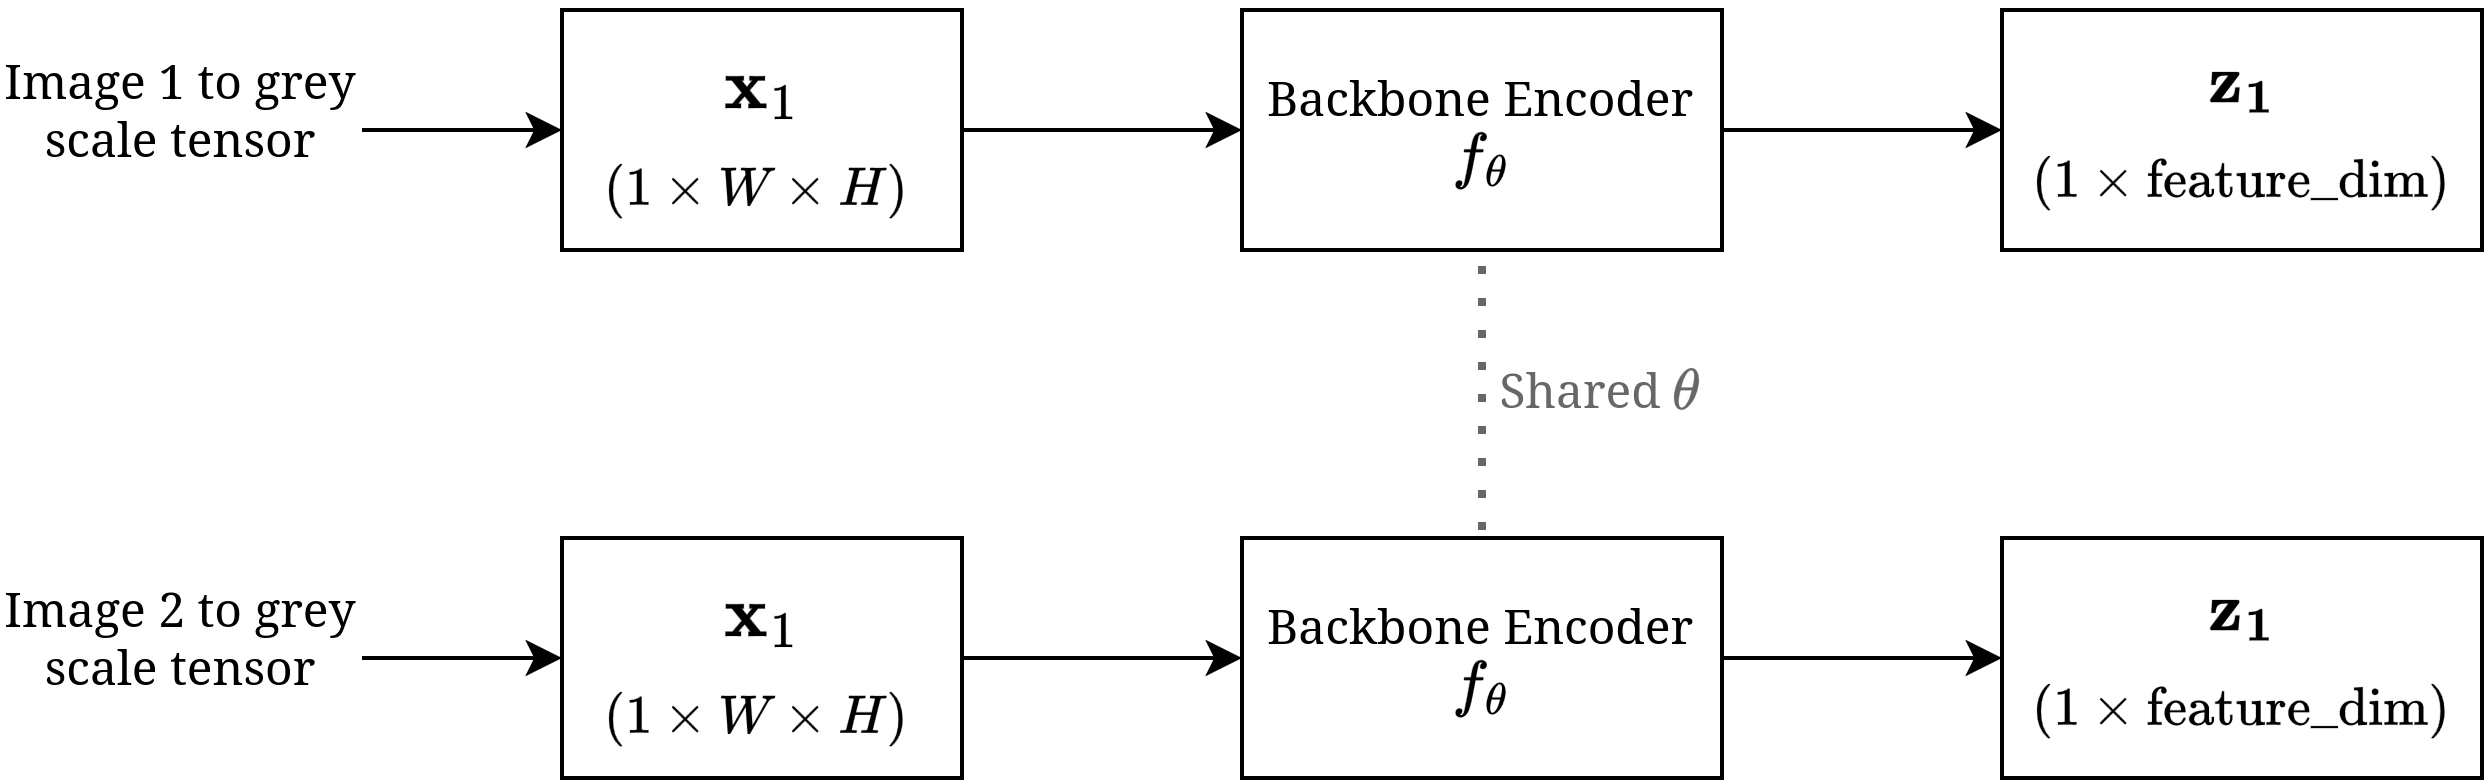
\includegraphics[width=0.8\textwidth]{images/siamese-architecture.drawio.png}
    \caption{Overview of the encoder architecture up to the feature dimension.}
    \label{fig:encoder-architecture}
\end{figure}
% 


Our framework implements a modular Siamese architecture composed of three main components: the backbone encoder, the projection head, and the decision mechanism. All components utilize shared weights between the twin networks to ensure symmetric feature extraction.

\subsubsection{Backbone Encoder}

The backbone encoder extracts high-level discriminative features from input handwriting images. We systematically evaluate six state-of-the-art convolutional neural network architectures organized into three architectural families:

\begin{itemize}
\item \textbf{ResNet family:} ResNet18 and ResNet34 with residual connections for deep feature learning
\item \textbf{EfficientNet family:} EfficientNet-B0 and EfficientNet-B1 employing compound scaling strategies
\item \textbf{MobileNet family:} MobileNetV3-Small and MobileNetV3-Large utilizing depthwise separable convolutions for efficiency
\end{itemize}

All backbones are initialized with ImageNet pre-trained weights to leverage transfer learning from large-scale visual recognition tasks. To adapt RGB-pretrained models to grayscale handwriting inputs while preserving the learned representations, the first convolutional layer is not reinitialized. Instead, the pretrained convolutional filters corresponding to the three RGB input channels are aggregated into a single-channel representation.

Specifically, given the original first convolutional layer:

\begin{equation}
\text{Conv2d}(3, C_{\text{out}}, \text{kernel\_size}, \text{stride}, \text{padding}, \text{bias}=\text{False}),
\end{equation}

the weights of the three input channels are averaged to produce a single-channel kernel:

\begin{equation}
W_{\text{gray}} = \frac{1}{3} \sum_{c=1}^{3} W_c,
\end{equation}

where $W_c$ denotes the pretrained weights associated with the $c$-th RGB channel.  
The resulting weights are then used to define a grayscale-compatible convolutional layer:

\begin{equation}
\text{Conv2d}(1, C_{\text{out}}, \text{kernel\_size}, \text{stride}, \text{padding}, \text{bias}=\text{False}),
\end{equation}

thereby retaining the pretrained knowledge of the original model while enabling processing of single-channel input images.

\subsubsection{Head Networks}

Depending on the training objective, different head architectures are employed on top of the shared backbone encoder.

\paragraph{Similarity (Decision) Head for BCE Models}

For BCE-based Siamese models, verification is formulated as a binary classification problem. Given two input images, the encoder produces two feature embeddings:

\begin{equation}
\mathbf{z}_1,\mathbf{z}_2 \in \mathbb{R}^{D}
\end{equation}

where $D$ denotes the embedding dimensionality. The two embeddings are concatenated to form the input representation of the decision head:

\begin{equation}
\mathbf{h}^{(0)}
=
[\mathbf{z}_1;\mathbf{z}_2]
\in
\mathbb{R}^{2D}
\end{equation}

The decision head is implemented as a fully connected network with progressively reduced dimensionality:

\begin{equation}
\mathbb{R}^{2D}
\rightarrow
\mathbb{R}^{32}
\rightarrow
\mathbb{R}^{16}
\rightarrow
\mathbb{R}^{8}
\rightarrow
\mathbb{R}^{4}
\rightarrow
\mathbb{R}^{2}
\rightarrow
[0,1]
\end{equation}

Each hidden layer applies a linear transformation followed by batch normalization\cite{ioffe2015batchnorm}, ReLU activation, and dropout regularization. The generic transformation is defined as:

\begin{equation}
\mathbf{h}^{(l+1)}
=
\mathrm{Dropout}_{p_l}
\left(
\mathrm{ReLU}
\left(
\mathrm{BN}
\left(
\mathbf{W}^{(l)}\mathbf{h}^{(l)}
+
\mathbf{b}^{(l)}
\right)
\right)
\right)
\end{equation}

where:

\begin{equation}
\mathbf{W}^{(l)}
\in
\mathbb{R}^{d_{l+1}\times d_l},
\qquad
\mathbf{b}^{(l)}
\in
\mathbb{R}^{d_{l+1}}
\end{equation}

and $d_l$ and $d_{l+1}$ denote the input and output dimensionalities of the $l$-th fully connected layer.

The dropout probabilities applied after each hidden layer are:

\begin{equation}
p_l \in \{0.20,0.20,0.18,0.16,0.12\}
\end{equation}

After the final hidden representation:

\begin{equation}
\mathbf{h}^{(5)}\in\mathbb{R}^{2}
\end{equation}

the last linear layer produces a scalar logit:
\begin{equation}
a
=
\mathbf{W}^{(5)}\mathbf{h}^{(5)}
+
b^{(5)}
\end{equation}
where:
\begin{equation}
\mathbf{W}^{(5)}\in\mathbb{R}^{1\times2},
\qquad
b^{(5)}\in\mathbb{R}
\end{equation}

The final similarity score is obtained through a sigmoid activation:

\begin{equation}
\hat{y}
=
\sigma(a)
=
\frac{1}{1+e^{-a}}
\end{equation}

where:

\begin{equation}
\hat{y}\in(0,1)
\end{equation}

represents the predicted probability that the two input images belong to the same writer.

Unlike metric-learning approaches, this BCE-based decision head does not explicitly
enforce geometric constraints on the embedding space. Instead, it learns a discriminative
similarity function directly from the concatenated encoder representations, as illustrated
in Figure~\ref{fig:bce-architecture}.

\begin{figure}[h!]
    \centering
    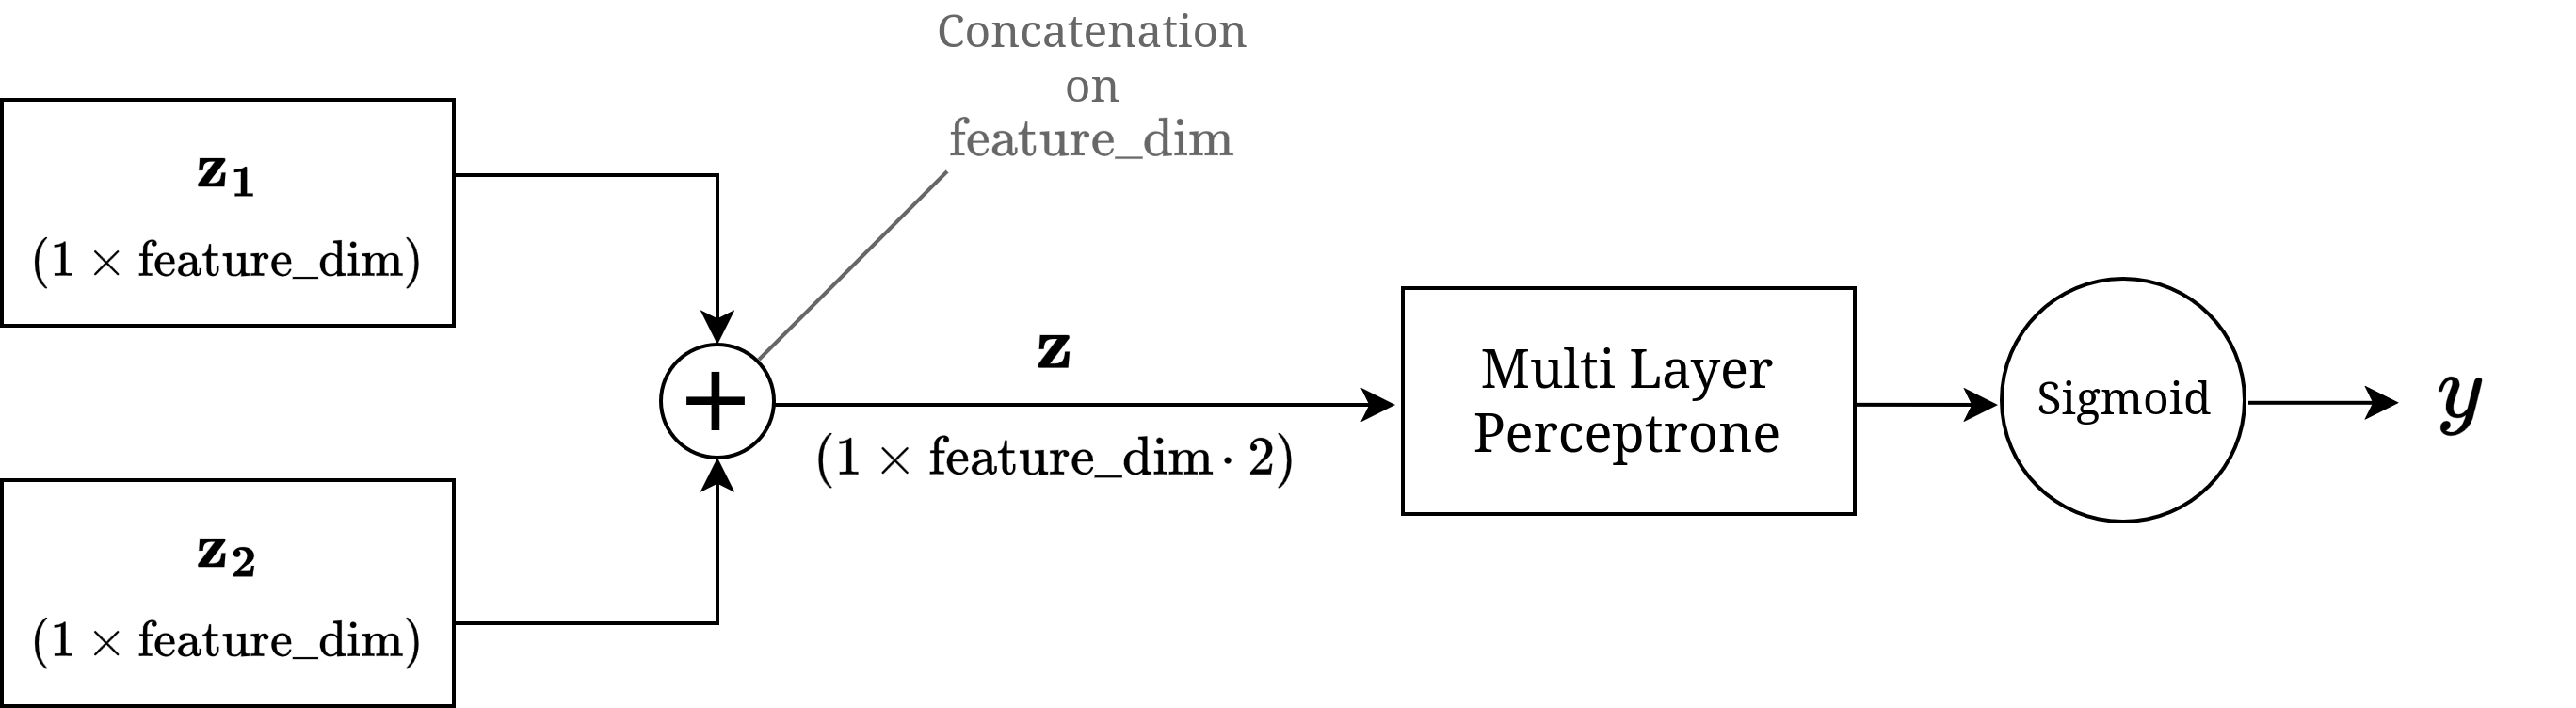
\includegraphics[width=1.0\textwidth]{images/bce-architecture.drawio.png}
    \caption{Similarity (decision) head for BCE-based models. The concatenated
    embeddings $\mathbf{z}_1$ and $\mathbf{z}_2$ are processed by a multi-layer
    perceptron followed by a sigmoid activation, producing a similarity score
    $\hat{y} \in (0,1)$.}
    \label{fig:bce-architecture}
\end{figure}

\paragraph{Projection Head for Contrastive and Triplet Models}

For contrastive and triplet learning objectives, the shared encoder extracts feature representations from two input images:

\begin{equation}
\mathbf{z}_1,\mathbf{z}_2\in\mathbb{R}^{D}
\end{equation}

where $D$ denotes the dimensionality of the backbone features. The two feature vectors are independently processed by the same projection head with shared parameters:

\begin{equation}
\mathbf{e}_1=g_{\phi}(\mathbf{z}_1),
\qquad
\mathbf{e}_2=g_{\phi}(\mathbf{z}_2)
\end{equation}

where $g_{\phi}$ denotes the MLP projection head and $\phi$ represents its learnable
parameters, as depicted in Figure~\ref{fig:contrastive-architecture}.

\begin{figure}[h!]
    \centering
    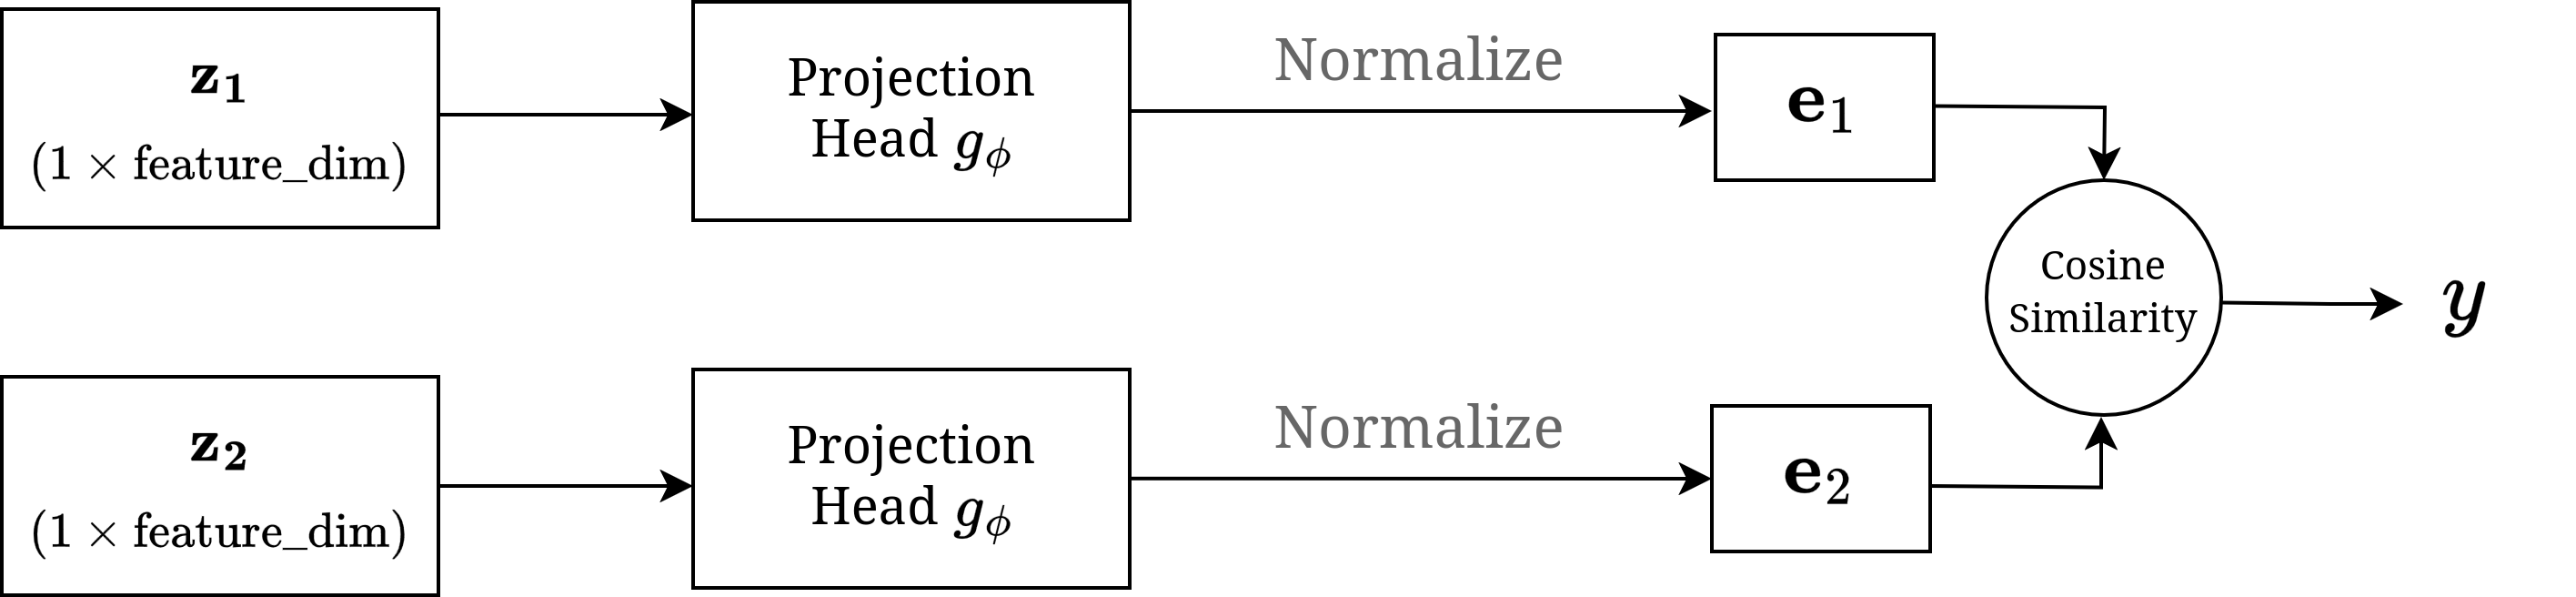
\includegraphics[width=1.0\textwidth]{images/contrastive-architecture.drawio.png}
    \caption{Projection head for contrastive and triplet learning models. Backbone
    features $\mathbf{z}_1$ and $\mathbf{z}_2$ are independently mapped by the shared
    projection head $g_\phi$, $\ell_2$-normalized, and compared via cosine similarity.}
    \label{fig:contrastive-architecture}
\end{figure}

The projection network maps the backbone features into a lower-dimensional embedding space according to:

\begin{equation}
\mathbb{R}^{D}
\rightarrow
\mathbb{R}^{1024}
\rightarrow
\mathbb{R}^{512}
\rightarrow
\mathbb{R}^{256}
\rightarrow
\mathbb{R}^{32}
\end{equation}

Each hidden layer applies a linear transformation followed by batch normalization, 
ReLU activation, and dropout regularization:

\begin{equation}
\mathbf{h}^{(l+1)}
=
\mathrm{Dropout}_{p_l}
\left(
\mathrm{ReLU}
\left(
\mathrm{BN}
\left(
\mathbf{W}^{(l)}
\mathbf{h}^{(l)}
+
\mathbf{b}^{(l)}
\right)
\right)
\right)
\end{equation}

where:

\begin{equation}
\mathbf{W}^{(l)}
\in
\mathbb{R}^{d_{l+1}\times d_l},
\qquad
\mathbf{b}^{(l)}
\in
\mathbb{R}^{d_{l+1}}
\end{equation}

The final projection layer produces the 32-dimensional embedding without applying any non-linear activation:

\begin{equation}
\mathbf{e}_i
=
\mathbf{W}^{(3)}
\mathbf{h}^{(3)}_i
+
\mathbf{b}^{(3)},
\qquad i\in\{1,2\}
\end{equation}

The resulting embeddings are normalized independently using $\ell_2$ normalization:

\begin{equation}
\hat{\mathbf{e}}_i
=
\frac{\mathbf{e}_i}
{\|\mathbf{e}_i\|_2},
\qquad i\in\{1,2\}
\end{equation}

obtaining unit-length embeddings:

\begin{equation}
\hat{\mathbf{e}}_1,\hat{\mathbf{e}}_2\in\mathbb{R}^{32},
\qquad
\|\hat{\mathbf{e}}_1\|_2=\|\hat{\mathbf{e}}_2\|_2=1
\end{equation}

The dropout probabilities applied after the hidden layers are:

\begin{equation}
p_l\in\{0.20,0.20,0.16\}
\end{equation}

The two normalized embeddings are then compared through cosine similarity:

\begin{equation}
s_{12}
=
\frac{\hat{\mathbf{e}}_1^T\hat{\mathbf{e}}_2}
{\|\hat{\mathbf{e}}_1\|_2\|\hat{\mathbf{e}}_2\|_2}
\end{equation}

Since the embeddings are normalized:

\begin{equation}
s_{12}=\hat{\mathbf{e}}_1^T\hat{\mathbf{e}}_2
\end{equation}

For contrastive learning, the similarity score is optimized directly by minimizing the distance between genuine pairs and enforcing a margin separation between impostor pairs.

For triplet learning, the same shared embedding function is applied to additional samples during training. The resulting embeddings are compared through relative similarities, enforcing that the anchor-positive similarity is larger than the anchor-negative similarity by a margin:

\begin{equation}
s_{ap}>s_{an}+m
\end{equation}

Therefore, both approaches use the same shared projection architecture and produce normalized embeddings suitable for metric comparison. The difference lies only in the optimization objective: contrastive learning operates on pairs of embeddings, whereas triplet learning optimizes relative relationships among anchor, positive, and negative samples.

\subsection{Loss Functions}

We investigate three loss formulations representing different approaches to the verification problem:

\subsubsection{Binary Cross-Entropy Loss}

BCE treats verification as direct similarity classification:
\begin{equation}
\mathcal{L}_{\text{BCE}} = -\frac{1}{N}\sum_{i=1}^{N} \left[y_i \log(\hat{y}_i) + (1-y_i)\log(1-\hat{y}_i)\right]
\end{equation}

where $\hat{y}_i \in [0,1]$ is the predicted similarity score and $y_i \in \{0,1\}$ is the ground truth label. This formulation provides stable gradients and reliable convergence but does not explicitly structure the embedding space according to metric properties.

\subsubsection{Contrastive Loss}

Contrastive Loss explicitly optimizes pairwise distances with margin-based separation:
\begin{equation}
\mathcal{L}_{\text{Contrastive}} =
\frac{1}{N}\sum_{i=1}^{N}
\left[
y_i d_i^2 +
(1-y_i)\max(m-d_i,0)^2
\right]
\end{equation}

where $d_i = 1-s_i$ represents the cosine-based distance derived from the cosine similarity $s_i$, and $m$ is the margin hyperparameter. The cosine similarity is computed between L2-normalized feature embeddings, resulting in $s_i \in [-1,1]$ and $d_i \in [0,2]$. Genuine pairs ($y_i=1$) minimize the distance between embeddings, while impostor pairs ($y_i=0$) are penalized when their distance falls below the margin threshold $m$, encouraging separation in the embedding space. We set $m=1.0$ based on preliminary experiments.

\subsubsection{Triplet Loss}

Triplet Loss enforces relative distance constraints by optimizing the separation between anchor-positive and anchor-negative pairs. Given a triplet composed of an anchor sample, a positive sample from the same writer, and a negative sample from a different writer, the loss is defined as:

\begin{equation}
\mathcal{L}_{\text{Triplet}} =
\frac{1}{N}\sum_{i=1}^{N}
\max\left(d_{ap}^{(i)} - d_{an}^{(i)} + m, 0\right)
\end{equation}

where $d_{ap}$ and $d_{an}$ denote the cosine distances between the anchor-positive and anchor-negative embeddings, respectively. The cosine distance is defined as:

\begin{equation}
d(x,y)=1-\cos(x,y)
\end{equation}

where cosine similarity is computed between L2-normalized embeddings, resulting in $d(x,y) \in [0,2]$. The loss encourages the distance between samples from the same writer to be smaller than the distance between samples from different writers by at least a margin $m$. When the constraint

\begin{equation}
d_{ap} + m < d_{an}
\end{equation}

is satisfied, the contribution to the loss becomes zero, meaning that the triplet already satisfies the desired separation. We set $m=0.5$ based on preliminary experiments, providing a balance between intra-class compactness and inter-class separation.

\subsection{Training Strategies}

\subsubsection{Dynamic Negative Sampling}

Class imbalance poses a significant challenge in writer verification \cite{he2009imbalanced}.
Given $W$ writers with $N_w$ samples each, the number of genuine pairs scales as
$O(W \cdot N_w^2)$ while impostor pairs scale as $O(W^2 \cdot N_w^2)$, creating severe
imbalance with impostor pairs vastly outnumbering genuine pairs.

We address this through epoch-wise dynamic negative resampling, a random undersampling
strategy applied to the majority class \cite{he2009imbalanced}. All genuine pairs are
preserved (being the minority class), while impostor pairs are randomly resampled each
epoch to maintain a target positive ratio. This strategy exposes the model to diverse
negative examples across epochs while maintaining balanced training signals:

\begin{algorithm}[H]
\caption{Dynamic Negative Sampling Strategy}
\begin{algorithmic}[1]
\State Generate all genuine pairs $\mathcal{P}_{\text{genuine}}$ from same-writer samples
\State Generate complete pool of impostor pairs $\mathcal{P}_{\text{impostor}}$
\State Compute required impostor count: $N_{\text{imp}} = \lfloor N_{\text{gen}} \cdot (1-r)/r \rfloor$
\For{epoch $e = 1$ to $E$}
    \State Sample $\mathcal{P}_{\text{impostor}}^{(e)} \subset \mathcal{P}_{\text{impostor}}$ with $|\mathcal{P}_{\text{impostor}}^{(e)}| = N_{\text{imp}}$
    \State $\mathcal{D}^{(e)} = \mathcal{P}_{\text{genuine}} \cup \mathcal{P}_{\text{impostor}}^{(e)}$
    \State Shuffle $\mathcal{D}^{(e)}$
    \State Train on $\mathcal{D}^{(e)}$
\EndFor
\end{algorithmic}
\end{algorithm}

where $r$ is the target positive ratio (set to 0.5 for balanced training).

\subsubsection{Selective Layer Freezing}

To prevent overfitting on limited handwriting data while maintaining transfer learning benefits, 
we implement selective layer freezing in the backbone encoder. The first $L_f$ convolutional 
layers remain frozen with gradients disabled, preserving generic low-level features learned from ImageNet, 
while deeper layers undergo fine-tuning for task-specific adaptation:

\begin{equation}
\theta = \{\theta_{\text{frozen}}, \theta_{\text{trainable}}\}, \quad \text{where} \quad \frac{\partial \mathcal{L}}{\partial \theta_{\text{frozen}}} = 0
\end{equation}

We freeze $L_f = 3$ initial layers for all backbone architectures trained, striking a balance between preserving pretrained knowledge and allowing 
domain adaptation.

\subsubsection{Regularization Techniques}

To prevent overfitting, we employ a comprehensive regularization strategy:

\begin{itemize}
\item \textbf{Graduated Dropout:} Starting from a base rate of $0.2$, dropout is scaled by a per-layer factor (1.0, 1.0, 0.9, 0.8, 0.6) so that deeper layers retain more expressiveness. This yields rates of $\{0.20,0.20,0.18,0.16,0.12\}$ for the five-layer BCE decision head and $\{0.20,0.20,0.16\}$ for the three-layer contrastive/triplet projection head.
\item \textbf{Weight Decay:} Decoupled weight decay (as implemented by AdamW) with coefficient $\lambda = 10^{-4}$ applied to all trainable parameters prevents weight magnitude explosion.
\item \textbf{Batch Normalization:} Applied after each linear transformation to stabilize training dynamics and provide implicit regularization through mini-batch statistics.

\item \textbf{Data Augmentation:} Training images undergo random transformations including rotation ($\pm15°$) and random resized crops (90-110\% of original size) to simulate natural writing variations while preserving character structure.
\end{itemize}

\subsection{Optimization}

We employ the AdamW\cite{loshchilov2019adamw} optimizer with hyperparameters adapted to model capacity:

\begin{equation}
\text{lr} = \begin{cases}
5 \times 10^{-5} & \text{if } |\theta| > 15 \times 10^6 \\
1 \times 10^{-4} & \text{otherwise}
\end{cases}
\end{equation}

where $|\theta|$ denotes the total number of trainable parameters. Additional optimizer parameters are set to $\beta_1 = 0.9$, $\beta_2 = 0.999$, $\epsilon = 10^{-8}$, and weight decay $\lambda = 10^{-4}$.

Learning rate scheduling employs ReduceLROnPlateau with factor 0.5 and patience 2 epochs, monitoring validation loss for dynamic adaptation. Early stopping with patience 5 epochs prevents overfitting while allowing sufficient convergence time, terminating training when validation loss fails to improve for the patience period.